\section{Problem Modeling}
\label{sec:model}

For a prescribed number $N$ of identical turbines with rotor radius $R$ (diameter $D=2R$), the $n=2N$ coordinates of the layout $\mathbf X=(x_1,y_1,\ldots,x_N,y_N)$ are optimized to maximize the expected farm power, i.e., to minimize the wake loss, under the Jensen wake model~\cite{Jensen1983,Katic1986} and the power curve of~\cite{Kusiak2010}. The wind direction $\theta$ has the probability density $p_\theta$; it is the direction \emph{towards} which the wind blows, counter-clockwise from east (Fig.~\ref{fig:model}a); the meteorological directions $\theta_{\rm met}$ of Horns Rev~1 and IEA37 (wind \emph{from}, clockwise from north) are converted by $\theta=270^\circ-\theta_{\rm met}$. Two constraints apply (Section~\ref{sec:constraints}): the turbine distances $\ell_{ij}=\lVert(x_i-x_j,\,y_i-y_j)\rVert_2$ are at least $\ell_{\min}=4D=8R$~\cite{Kusiak2010,Bansal2017}, and the farm is a disc of radius $r=500$, 750 or 1000~m. The spacing $4D$ is the convention of the Kusiak--Song benchmark and is kept for comparability; it lies at the dense end of practice (the installed Horns Rev~1 layout is a regular grid of about $7D$; Section~\ref{sec:hornsrev-site}), so our results concern a packing-constrained regime (larger spacings: Section~\ref{sec:spacing}).

The model is the unchanged Kusiak--Song benchmark model, and no modeling novelty is claimed; the contributions are the PSO-VNS algorithm and its controlled evaluation. The terrain is flat, and the electrical collector-system layout and multi-objective formulations (e.g., AEP against cost or the levelized cost of energy) are not considered. The protocol (equal budgets, seed pairing, equal-cost controls, feasibility-aware ranking, equivalence tests) does not depend on the model and applies to such formulations as well.

\begin{figure}[!t]
\centering
\begin{minipage}[b]{0.26\textwidth}\centering
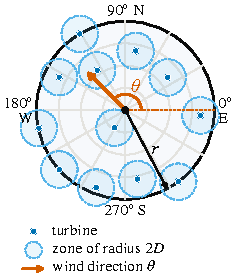
\includegraphics[width=\linewidth]{figures_final/fig_wind_farm.pdf}\\[-2pt]{\small (a)}
\end{minipage}\hfill
\begin{minipage}[b]{0.35\textwidth}\centering
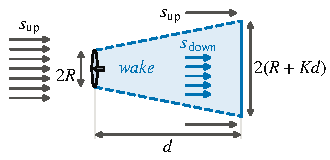
\includegraphics[width=\linewidth]{figures_final/fig_wake_model.pdf}\\[4pt]{\small (b)}
\end{minipage}\hfill
\begin{minipage}[b]{0.35\textwidth}\centering
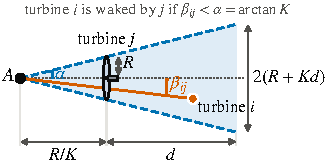
\includegraphics[width=\linewidth]{figures_final/fig_half_cone.pdf}\\[4pt]{\small (c)}
\end{minipage}
\caption{Model geometry. (a) Circular farm of radius $r$ and wind direction $\theta$; the points show, for illustration, a 12-turbine layout ($r=750$~m); discs of radius $2D$ touch at the spacing $\ell_{\min}=4D$. (b) Jensen top-hat wake behind a rotor of radius $R$: width $2(R+Kd)$ at the downstream distance $d$, uniform speed $s_{\text{down}}<s_{\text{up}}$. (c) Wake half cone of turbine $j$ ($K$ exaggerated): virtual vertex $A$ at $R/K$ upstream of the rotor, half-angle $\alpha=\arctan K$; turbine $i$ is waked by $j$ if $\beta_{ij}<\alpha$.}
\label{fig:model}
\label{fig:S-farm}\label{fig:S-wake}\label{fig:S-halfcone}
\end{figure}

\subsection{Wind Model and Direction Discretization}
\label{sec:wind}
For each direction, the wind speed $s$ has the Weibull density $p_s(s;\zeta,\psi)=(\zeta/\psi)\allowbreak(s/\psi)^{\zeta-1}\allowbreak\exp[-(s/\psi)^{\zeta}]$ with shape $\zeta(\theta)$ and scale $\psi(\theta)$. The benchmark rose is piecewise constant: $N_\theta=24$ direction bins $[15(l-1),15l)^\circ$, $l=1,\ldots,24$, with probability $p_l$, shape $\zeta=2$ and scale $\psi_l$ (Table~\ref{S-tab:S-wind}). Data Set~I is nearly unidirectional ($\psi=13$~m/s in all bins; 80\% of the probability in bins 6 and 7, i.e., wind from 165$^\circ$ to 195$^\circ$); Data Set~II is a broad rose with scales from 2.6 to 10~m/s and its highest probability in bin~13. Both are synthetic wind roses of the Kusiak--Song benchmark~\cite{Kusiak2010,Bansal2017}, not measurements at a site; the measured wind climates in this study are the 12-sector Weibull roses of the Horns Rev~1 block (Section~\ref{sec:hornsrev-site}) and of a Lillgrund block (Section~\ref{sec:lillgrund}), both optimized in 5$^\circ$ bins, and IEA37 Case Study~1 uses 16 directions at one speed (Section~\ref{sec:setup-beyond}).
% verified: analysis/wflop_model.py (DS1_W, DS1_PSI, DS2_PSI, DS2_W; k = 2); bins 6+7 of DS I: 0.2+0.6 = 0.8, towards 75-105 deg = from 165-195 deg

\emph{Why the direction discretization matters.} The objective evaluates the wake only at the 24 bin centers $\bar\theta_l=(15l-7.5)^\circ$. A top-hat wake is narrow: by the half-cone geometry (Fig.~\ref{fig:model}c), turbine $j$ wakes a turbine $i$ at the distance $\rho\ge R/K$ only for directions within an interval of width $2[\alpha+\arcsin(R/(\rho\sqrt{1+K^2}))]$ around the direction from $j$ to $i$. With $K=0.075$ and $R=38.5$~m ($\alpha=4.29^\circ$, $R/K=513$~m), this width is below the bin spacing of 15$^\circ$ for $\rho>685$~m and tends to $2\alpha=8.6^\circ$. If no bin center lies in this interval, the wake of the pair does not enter the objective (with bins of 5$^\circ$ or finer, every such interval contains a center). Optimized layouts exploit these gaps (with 1$^\circ$ sub-bins, the mean wake loss of PSO-VNS rises by about 1~pp); Section~\ref{sec:direction} reports which conclusions survive a 1$^\circ$ rose, for re-evaluated and for directly optimized layouts.
% verified (numerically with analysis/wflop_model.jensen_deficits on a 0.001-deg grid): waked width of a pair rho apart = 2(alpha + arcsin(R/(rho sqrt(1+K^2)))) exactly for rho >= R/K (rho = 600: 15.915 deg; 1000: 12.979; 2000: 10.779); width = 15 deg at rho = 685.4 m; alpha = arctan 0.075 = 4.289 deg; R/K = 513.3 m; 2 alpha = 8.58 deg > 5 deg. For rho < R/K the non-physical upstream deficit widens the interval further.
% CHECK-DIR [F03]: loss rise of every method, PSO-VNS 1.322 -> 2.335; [F05]: VNS-based methods and PSO rise most

\subsection{Wake Effect Model}
In the Jensen model (Fig.~\ref{fig:model}b,c), the wake of turbine $j$ is a half cone with half-angle $\alpha=\arctan K$ (wake-spreading constant $K$), and its virtual vertex lies $R/K$ upstream of the rotor. With $u_{ij}=(x_i - x_j)\cos\theta + (y_i - y_j)\sin\theta + R/K$ and the lateral offset $v_{ij}=-(x_i - x_j)\sin\theta + (y_i - y_j)\cos\theta$, turbine $i$ lies in the wake if $\beta_{ij}=\cos^{-1}\!\bigl(u_{ij}/\sqrt{u_{ij}^2+v_{ij}^2}\bigr)<\alpha$. Its downstream distance is $d_{ij}=\lvert u_{ij}-R/K\rvert$, and with the thrust coefficient $C_T$ the velocity deficit is
\begin{equation}
    \Delta_{ij} = 1-\frac{s_{\text{down}}}{s_{\text{up}}}=\frac{1 - \sqrt{1 - C_T}}{\left(1 + K d_{ij}/R\right)^2}.
    \label{eq:deficit}
\end{equation}
The numerator is the deficit behind the rotor from actuator-disc momentum theory, and the factor $R^2/(R+Kd_{ij})^2$ spreads it over the growing wake (Fig.~\ref{fig:model}b); with $C_T=0.8$ and $K=0.075$, a turbine $\ell_{\min}=308$~m directly behind another loses 21.6\% of the wind speed, one 770~m ($10D$) behind 8.8\%.
% verified: (1-sqrt(0.2))/(1+0.075*308/38.5)^2 = 0.2159; (1-sqrt(0.2))/(1+0.075*770/38.5)^2 = 0.0884
As in~\cite{Kusiak2010}, this top-hat wake is tested at the hub center only, so the deficit jumps at the cone edge, and it also reaches a turbine less than $R/K$ \emph{upstream} of $j$ near its axis (between $A$ and the rotor in Fig.~\ref{fig:model}c; non-physical, kept for comparability with the published results). The deficits are combined by the root-sum-square rule,
\begin{equation}\label{eq5}
\Delta_i(\theta) = \Bigl( \textstyle\sum_{j \ne i,\ \beta_{ij} < \alpha} \Delta_{ij}^2 \Bigr)^{1/2} .
\end{equation}
As $C_T$ is constant (which overstates the deficits above rated speed), $\Delta_i(\theta)$ depends only on the layout and the direction, not on the free-stream speed $s$; the local wind speed in a direction bin, $s_{\rm local}=[1-\Delta_i(\theta)]\,s$, is therefore a scaled Weibull variable, with the same shape $\zeta(\theta)$ and the scale $\psi_i(\theta)=\psi(\theta)[1-\Delta_i(\theta)]$. The Horns Rev~1 model (Section~\ref{sec:hornsrev-site}) instead takes $C_T$ from the V80 thrust curve at the free-stream speed of each 1-m/s speed bin and sums the power over these bins, so it does not use this scaling (Section~\ref{S-sec:S-hrmodel}). The hub-center test makes the objective jump where a hub crosses a cone edge in an evaluated direction; hence the derivative-free local search of VNS (Section~\ref{sec:vns}), and finite-difference gradients handicap MS-SLSQP.

\emph{Why the Jensen model.} First, the Jensen model with the benchmark settings is needed for comparability with the published Kusiak--Song results~\cite{Kusiak2010,Bansal2017}, and it is cheap enough for the 52{,}930 optimization runs of this study (Table~\ref{tab:design}). Second, the research question concerns the optimizers and the protocol rather than the fidelity of the wake model; whether the conclusions carry over to another wake model is an empirical question. Third, we therefore test a Gaussian wake in two ways: the methods are re-optimized under the simplified Bastankhah Gaussian wake of IEA37 Case Study~1 (Section~\ref{sec:iea37}), and the final benchmark layouts are re-evaluated with the Gaussian wake of~\cite{Bastankhah2014} (Section~\ref{sec:gaussian}). Control-oriented models, which describe the wake deflection of yawed turbines for wake steering~\cite{Gebraad2016,Bastankhah2016}, add yaw angles as decision variables and turn the problem into a layout--control co-design, which is outside the scope of this study.

\subsection{Power Model and Expected Energy}
\label{sec:powermodel}
\label{sec:S-power}
The power curve of the Kusiak--Song benchmark~\cite{Kusiak2010} is $f(s)=0$ for $s<s_{\text{cut-in}}$, $f(s)=\lambda_1 s+\lambda_0$ for $s_{\text{cut-in}}\le s\le s_{\text{rated}}$ and $f(s)=P_{\text{rated}}$ above, with $s_{\text{cut-in}}=3.5$~m/s, $s_{\text{rated}}=14$~m/s, $P_{\text{rated}}=1500$~kW, $\lambda_1=140.86$ and $\lambda_0=-500$. We use it as published: it is slightly negative just above the cut-in speed ($-7.0$~kW at 3.5~m/s, zero at 3.55~m/s), jumps from 1472 to 1500~kW at the rated speed and has no cut-out speed. We keep this linearized curve for comparability with the published Kusiak--Song results; its effect on the energy values is quantified with a cubic curve in Section~\ref{sec:powercurve}, and the Horns Rev~1 block uses the tabulated V80 power curve (Section~\ref{sec:hornsrev-site}). The expected power of turbine $i$,
\begin{equation}\label{eq8}
E(P_i) = \int_0^{360} p_\theta(\theta) \int_0^{\infty} f(s)\,
       p_s\bigl(s; \zeta(\theta), \psi_i(\theta)\bigr) \, ds \, d\theta ,
\end{equation}
is evaluated, as in~\cite{Kusiak2010}, by a Riemann sum over direction bins $\theta_0 = 0^\circ, \theta_1, \ldots, \theta_{N_\theta} = 360^\circ$ with probabilities $p_l$, and over the speed range between $s_{\text{cut-in}}$ and $s_{\text{rated}}$, divided into $N_s$ bins $s_0 = s_{\text{cut-in}}, s_1, \ldots, s_{N_s} = s_{\text{rated}}$ (benchmark: $N_\theta=24$ bins of 15$^\circ$ and $N_s=21$ bins of 0.5~m/s). With the bin centers $\bar\theta_l=(\theta_{l-1}+\theta_l)/2$ and the Weibull survival function $W_i(s,\theta)=\exp\{-[s/\psi_i(\theta)]^{\zeta(\theta)}\}$ of the local speed,
\begin{equation}
\begin{split}
E(P_i) ={}& \sum_{l=1}^{N_\theta} (\theta_l - \theta_{l-1})\, p_l \Bigg\{ P_{\text{rated}}\, W_i(s_{\text{rated}},\bar\theta_l)
+\lambda_1 \sum_{q=1}^{N_s} \tfrac{s_{q-1} + s_q}{2}\bigl[W_i(s_{q-1},\bar\theta_l)-W_i(s_q,\bar\theta_l)\bigr]\\
&\qquad+ \lambda_0 \bigl[W_i(s_{\text{cut-in}},\bar\theta_l)-W_i(s_{\text{rated}},\bar\theta_l)\bigr] \Bigg\}.
\end{split}
\label{eq:S-power}
\end{equation}
Like the earlier studies, we keep the bin-width factor $(\theta_l-\theta_{l-1})$ in degrees; with 24 bins of $15^\circ$ and $\sum_l p_l=1$, the benchmark objective $\sum_i E(P_i)$ is thus 15 times the expected farm power in kW, and the gross (wake-only) annual energy production is $\mathrm{AEP}\,[\mathrm{MWh}] = (\text{objective}/15)\times 8.76$. The wake-free benchmark objective of one turbine, $E_{\rm ideal}$, is~\eqref{eq:S-power} with $\psi_i=\psi$; for Data Set~I, $E_{\rm ideal}=14{,}045.74$, which corresponds to 936.38~kW (a capacity factor of 62\%, far above real sites) or 8,202.7~MWh/yr.
% verified: 14045.74/15 = 936.38 kW; 936.38/1500 = 0.624; 936.38*8.76 = 8202.7 MWh (reproduced from wflop_model.py); N_s = (14-3.5)/0.5 = 21 (wflop_model.expected_power_linear); 140.86*3.5-500 = -6.99; 500/140.86 = 3.55; 140.86*14-500 = 1472.0

\subsection{Optimization Problem and Constraint Handling}
\label{sec:constraints}
With the wake loss $L(\mathbf X)=N E_{\rm ideal}-\sum_{i=1}^{N}E(P_i)$, reported in percent of the wake-free value, $100\,L/(NE_{\rm ideal})$, the problem is
\begin{equation}
\min_{\mathbf X\in[-r,r]^{2N}} L(\mathbf X)\quad\text{s.t.}\quad \ell_{ij}\ge\ell_{\min}\ (1\le i<j\le N),\qquad x_i^2+y_i^2\le r^2\ (1\le i\le N),
\label{eq:wflop}
\end{equation}
which is equivalent to maximizing the expected farm power and hence the AEP: a problem in $2N$ variables ($2N\le30$ on the benchmark) with a discontinuous objective and $N(N-1)/2$ nonconvex spacing constraints.
After every position update, each coordinate is clipped to $[-r,r]$ (box repair; the square, not the circle). The constraints are handled by a penalty on the violations $g^{\rm b}_{i}=x_i^2+y_i^2-r^2$ and $g^{\rm s}_{ij}=\ell_{\min}-\ell_{ij}$; all optimizers except MS-SLSQP minimize the penalized wake loss
\begin{equation}
\begin{split}
F_p(\mathbf X)={}&\Bigl(N E_{\rm ideal}-\sum_{i=1}^{N}E(P_i)\Bigr)+\sum_{i:\,g^{\rm b}_i>0}\bigl(1+\mu g^{\rm b}_i\bigr)^2\\
&+\sum_{i<j:\,g^{\rm s}_{ij}>0}\bigl(1+\mu g^{\rm s}_{ij}\bigr)^2,\qquad \mu=10^{10},
\end{split}
\label{eq:penalty}
\end{equation}
whose first term is the wake loss $L(\mathbf X)$ reported in our tables. Any violation above about $4.6\times10^{-8}$ (m or m$^2$) makes the penalty exceed any possible wake loss, so comparing $F_p$ values is, up to smaller violations, a feasibility-first rule (feasible before infeasible, then wake loss or total penalty). The scaling ($g^{\rm b}_i$ in m$^2$, $g^{\rm s}_{ij}$ in m) favors infeasible layouts with turbines slightly too close, or with a turbine clipped to the box near a tangent point $(\pm r,y_i)$, where $g^{\rm b}_i=y_i^2$. MS-SLSQP minimizes the wake loss under explicit constraints. A final layout counts as feasible if $\ell_{ij}\ge\ell_{\min}$ and $\sqrt{x_i^2+y_i^2}\le r$ hold within $10^{-6}$~m (Section~\ref{sec:setup}), a looser tolerance than the penalty's. With random starts, no optimizer guarantees a feasible final layout; infeasible final layouts are therefore counted, reported and ranked below feasible ones (Section~\ref{sec:setup-stats}). Section~\ref{sec:boundary} tests an alternative: Deb's feasibility rules~\cite{Deb2000} on dimensionless violations, with box clipping or radial projection.
% verified: largest benchmark wake loss < 15 x 14045.74 = 2.107e5 (plus the small negative part of f); (sqrt(2.2e5)-1)/1e10 = 4.6e-8
% CHECK-DIAG [D06]/[D21]: old-setting infeasible finals (1e-6 m rule) mostly spacing-only; boundary violations = turbine with a coordinate on the box bound (tangent-point pinning); numbers in 06_results sec:psosetting
